\chapter{背景}
    世界知名的亚马逊公司创建了在线市场并且为客户提供了对购买进行评级和审查的
机会。用户可以通过个人星级评级——从1星级到5星级来表示他们对产品的满意度,此外
,用户也可以通过提交文本信息来进行评论,从而进一步表达对待产品的看法和一些更
加具体的意见。用户除了直接针对商品进行评级和评价之外也可以针对其他用户的一些
评论进行评级,来表达他们认为这些评论是否对自己购买产品有帮助——从而使在线市场
能够筛选出有帮助的评论。

    而参与在线市场的产品营销公司则可以通过用户的各种数据数据来洞察他们是否应
该参与相关的市场和以及具体的参与时机,这也可以帮助他们对如何设计更受用户欢迎
的更成功的产品。

    如今,阳光公司正在计划在网上市场推出三种新产品:微波炉,婴儿奶嘴和吹风机。
他们聘请我们作为营销团队的顾问。要求我们通过过去用户提供的与其他竞争产品相关
的一些评论评级信息来为公司的在线销售战略提供信息,并且确定潜在的重要设计功能,
从而增强产品的受欢迎程度。公司曾经使用过数据来为销售战略提供信息,但是并没有
使用过特定的组合和类型的数据,他们表示对于这些数据中基于事件的模式非常感兴趣,
并且希望能够得到有助于公司制作出成功的产品的方式。
阳光数据中心为我们提供了这个项目的三个数据文件:\texttt{hair\_dryer.tsv},
\texttt{microwave.tsv}和\texttt{pacifier.tsv}。
这些数据包括了用户对亚马逊市场中销售的微波炉,婴儿安抚奶嘴和吹风机在一定时间段内的评级和评论信息,希
望我们通过这些数据,使用数据科学的相关方法,利用星级评级,评论和评论评级之间的关系和衡量标准等解决一
些具体问题或实现一些具体需求:
\begin{enumerate}
    \item 阳光公司的三种产品一旦在在线市场上线,希望能够根据评级和评论确定出最具信息量的数据衡量标准帮助公司跟踪
    \item 在每个数据集中识别并讨论基于时间的度量和模式,这些度量和模式可以表明产品在在线市场的声誉上升或下降
    \item 确定基于文本的衡量标准与基于评级的衡量标准的组合,从而能够更好的指示潜在的成功产品或失败产品
    \item 具体的星级评分能够带来怎样的影响,是否会引发更多的评论,客户在看到低星级评级后是否会撰写某种类型的评论
    \item 基于文本的评论的具体质量描述来判断其是否与评级等级息息相关
\end{enumerate}


\chapter{方法}
基于所提供的数据集,我们将每一条信息分为如下的维度:

\begin{description}
    \item [文本] 每一条评论的文字中都包含了丰富的语义信息。虽然文本信息是非结构
        化,非数字化的,但现在数据科学领域内有着大量成熟的{\fKai 自然语言处
        理}技术,通过一系列算法的变换后,可以得到包含语义信息的数值化数据。
    \item [时间] 商品的声誉并非是静态的,而是随着时间变化的。数据集中给出了每一
        条评论的时间戳,通过结合其他数据维度,可以获得数据之间的时序关联。
    \item [评分] 评分是用户对产品评价最基本的数值度量,平均评分也是最为容易取得
        的可靠指标。
    \item [评价数] 出于合理的推断,我们假设一个商品的评价量$C$总是占总销售量$S$的一
        个固定比例,即满足$C/S=\textrm{const}$。又因为销售量和产品营收成直接的正
        相关关系,所以评价数也可以作为一个重要的指标。
\end{description}

在经过基础的数据处理后,我们对不同维度的指标做交叉分析。基本的关系图
如\autoref{fig:schedule} 所示。

\begin{figure}
    \centering
    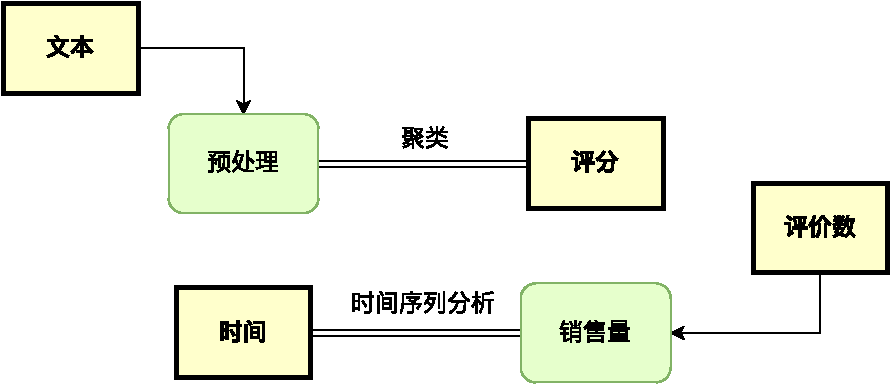
\includegraphics[width=0.8\textwidth]{main-relation.pdf}
    \caption{数据关系}
    \label{fig:schedule}
\end{figure}


\section{文本处理}

\begin{figure}
    \centering
    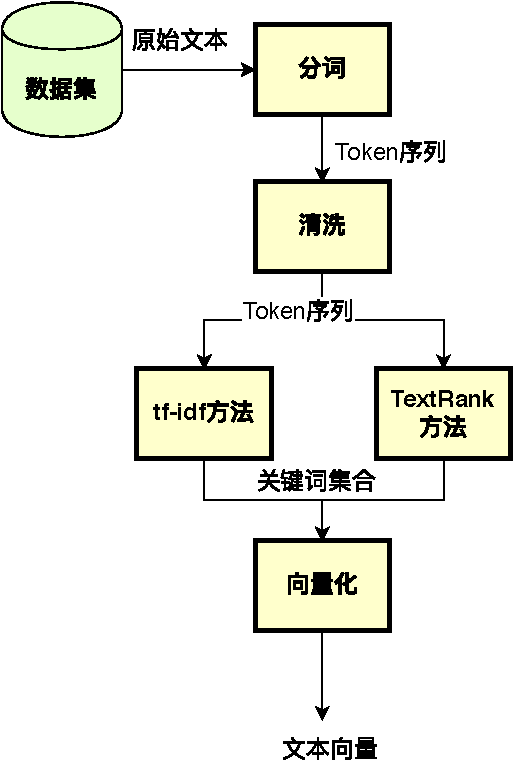
\includegraphics[width=0.4\textwidth]{text-process.pdf}
    \caption{文本处理流程}
    \label{fig:text-schedule}
\end{figure}

本文拟采用分词,关键字提取,文本向量化等方法对文本进行处理,以得到便于计算的向量
值。基本流程图见\autoref{fig:text-schedule}。

\subsection{分词(Tokenization)}
数据集中存在的文本是英文文本,可以使用一些英语的自然语言处理库来进行分词处理
经过分析与讨论,我们决定使用自然语言处理库NLTK\ucite{loper2002nltk}的\texttt{tokenize}函数来进行处理。
该函数和的分词方法和Penn TreeBank语料库的分词方法一致,TreeBank标记生成器使用正则表达式对文本进
行标记化。该过程由调用的方法\texttt{word\_tokenize()}。假设文本已经被分割成句子
,则使用\texttt{sent\_tokenize()}
来进行操作

该标记器执行以下步骤:
\begin{enumerate}
\item 分割标准收缩,例如将\texttt{don't}转化为\texttt{do n't}
\item 将大多数标点符号视为单独的标记进行分割
\item 分隔逗号和单引号以及句末的空格
\item 若出现了行末的单独的句点,将其分割开
\end{enumerate}

\subsection{文本清洗(Text Preprocessing)}
数据集中的用户评论文本是非结构化的复杂数据,有许多干扰因素。
在利用自然语言算法进行进一步处理之前,需要对文本进行清洗操作。

首先要去除非文本字符和标记。在文档中含有用于在网页上渲染格式的HTML标记
\texttt{<br/>},以及用于显示视频的\texttt{[[img:]]} 标记等。这些字符对于语义分析
和自然语言处理算法都没有价值,应当予以去除。

接下来考虑词汇的同一性的问题。英语单词在句首时需要大写首字母,但是这样的变化并不
带有语义信息;同时英语属于拉丁语系,单词具有不同的屈折变化(Inflection)。不同的
屈折变化语义相近,应该做合并处理。为了方便计算机处理,我们对单词做{\fKai
标准化} (Normalization)处理,将大写字母转换为小写,并使用NLTK库的{\fKai 词性还
原}功能进行处理。这样标准化之后的词汇可以直接用字符串比较来判断同一性。

最后,一个{\fKai 停用词表}(Stopwords List)给出了所有应该被去掉的虚词和信息量小
的实词。所有在该列表中的单词都被从文档中移除。本文使用了来自NLTK库的英语停用
词表,一共包含179个单词,见\autoref{fig:stopwords}。

\begin{figure}
    \noindent\fbox{
        \parbox[t]{1\columnwidth - 2\fboxsep - 2\fboxrule}{%
            \input{figures/stopwords.txt}
    }}
\caption{停用词表}\label{fig:stopwords}
\end{figure}

\subsection{关键词提取(Keyword Extraction)}
常见的关键词提取方法有tf-idf \ucite{ramos2003using},PageRank,Topic-model等算法。
本文使用tf-idf算法和PageRank算法的衍生算法TextRank算法\ucite{mihalcea2004textrank}来
进行关键词提取的操作。

\subsubsection{if-idf方法}

tf-idf是一种用于信息检索与数据挖掘的常用加权技术。tf是词频(Term Frequency),idf是
逆文本频率指数(Inverse Document Frequency)。它是一种统计方法,经常用来评估一字词对
于一个文件集或一个语料库中的其中一份文件的重要程度。字词的重要性随着它在文件中出现的
次数成正比增加,但同时会随着它在语料库中出现的频率成反比下降。tf-idf的主要思想是:如果
某个词或短语在一篇文章中出现的频率tf高,并且在其他文章中很少出现,则认为此词或者短语具
有很好的类别区分能力,适合用来分类。
其中tf的计算方法为:
\begin{equation}
    \mathrm{tf}_{\mathrm{i}, \mathrm{j}}=\frac{n_{i, j}}{\sum_{k} n_{k, j}}
\end{equation}
idf的计算方法为:
\begin{equation}
    \mathrm{idf}_{\mathrm{i}}=\lg \frac{|D|}{\left|\left\{j: t_{i} \in d_{j}\right\}\right|}
\end{equation}

分别计算出相应的tf和idf的值之后,将他们求积就可以得到对应的tf-idf值:
\begin{equation}
    \textrm{tfidf} _{i, j}=\textrm{tf}_{i, j} \times \textrm{idf}_{i}
\end{equation}

\subsubsection{TextRank方法}

PageRank设计之初用于Google的网页排名。其具体公式如下:
\begin{equation}
    S\left(V_{i}\right)=(1-d)+d \cdot \sum_{j \in \operatorname{In}\left(V_{i}\right)}
    \frac{1}{\lvert \operatorname{Out}\left(V_{j}\right)\rvert} S\left(V_{j}\right)
\end{equation}
该公式中,$V_{i}$表示某个网页,$V_{j}$表示链接到$V_{i}$的网页,$S\left(V_{i}\right)$
表示网页$V_{i}$的PR值,$I n\left(V_{i}\right)$表示网页Vi的所有入链的集合,$O u t\left(V_{j}\right)$

\begin{figure}
    \centering
    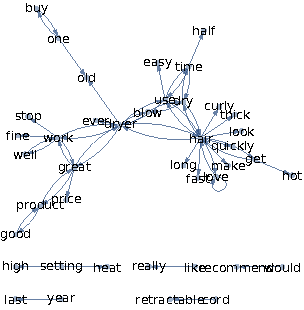
\includegraphics[scale=1.5]{figures/graph.pdf}
    \caption{关键词图$V$的一部分。{\fKai 选取了频数最大的20个元素,权值小于200的边被隐
    去。可以看出常见的词语组合如“last year”“buy one”等。}}
    \label{fig:textrank}
\end{figure}

我们使用了PageRank算法的衍生算法TextRank,与PageRank算法相比,它多了一个权重,用来表示
两个节点之间的边连接有不同的重要程度,迭代公式如下:
\begin{equation}\label{eq:textrank}
    W S\left(V_{i}\right)=(1-d)+d \cdot \sum_{V_{j} \in
    \operatorname{In}\left(V_{i}\right)} \frac{w_{j i}}{\sum_{V_{k} \in
\operatorname{Out}\left(V_{j}\right)} w_{j k}} W S\left(V_{j}\right)
\end{equation}

该算法的具体过程如下。
\begin{enumerate}
    \item 构建候选关键词图$G_K = (V,E)$,其中$V$为节点集,由上一步生成的候选关键词组成,然后采用共现关系构造任两点之间的边,
    两个节点之间存在边仅当它们对应的词汇在长度为$w$的窗口中共现,$w$表示窗口大小,
    即最多共现$w$个单词。关键词图的一部分见\autoref{fig:textrank} 。
    \item 根据\autoref{eq:textrank} ,迭代传播各节点的权重,直至收敛。
    \item 对节点权重进行倒序排序,从而得到最重要的$m'$个单词,构成集合$K'=\{K_j\}$
    %\item 上一步得到最重要的$T$个单词,在原始文本中进行标记,若他们能形成相邻词组,则组合成多词关键词也就是关键词组。
\end{enumerate}






\subsection{文本向量化}

基于提取的关键词,我们可以针对文档做文本向量化。文本向量化将由标记组成的
文本$T_n=\{t_1,t_2,\ldots,t_n\}$转换为向量$W_T=\{k_1,k_2,\ldots,k_m\}$,其中$n$为文
本的长度,$m$为向量的长度。为了找出关键词集合,首先需要选定一组序数为$m$
的关键词集合$K=\{K_i\}$,向量分量$k_i$为对应关键词在文章$T$中的tf-idf权重。
\begin{equation}
    k_i = \textrm{tfidf}_T(K_i)
\end{equation}
集合$K$由TextRank方法选出的关键字集合$K'$,再由tf-idf方法做反向筛选得出。
\begin{equation}
    K = \{K_i | K_i \in K', K_i \in \textrm{top 1000 of }K'_{\textrm{tfidf}} \}
\end{equation}

\section{评分与文本的关联聚类}
通过前面的步骤我们得到了一个数千维的向量$V$,为了进行接下来的聚类操作,我们决定先将这个高维
向量降维处理,结合课上所学内容,我们分析讨论之后决定使用主成分分析法(PCA)来进行降维操作。

PCA(Principal components analysis)是一种统计分析、简化数据集的方法。其具体实现步骤如下:
\begin{enumerate}
    \item 我们首先对特征进行归一化处理,以便于继续进行后面的操作
        \begin{equation}
            \left\{
            \begin{aligned}
                \mu_{j}&=\frac{1}{m} \sum_{i=1}^{m} x_{j}^{(i)} \\
                x_{j}^{(i)}&=x_{j}^{(i)}-\mu_{j} \\
                \sigma_{j}^{2}&=\frac{1}{m}
                \sum_{i=1}^{m}\left(x_{j}^{(i)}\right)^{2} \\
                x_{j}^{(i)}&=\frac{x_{j}^{(i)}}{\sigma_{j}} \\
            \end{aligned}
            \right.
        \end{equation}
    \item 计算协方差矩阵。\begin{equation}
        C=\frac{1}{m} X^{T} X
    \end{equation}
    \item 我们计算了向量的协方差矩阵的特征向量并按照特征大从大到小排序。
    \item 提取出特征向量矩阵的前$k$列。\begin{equation}
        U=\left(
            \boldsymbol u^{(1)} \quad \boldsymbol u^{(2)} \quad \cdots \quad \boldsymbol u^{(k)}
            \right)
    \end{equation}
    \item 通过矩阵乘法计算得到新的特征$Z$。\begin{equation}
            Z=X U=\left(\begin{array}{c}
            \boldsymbol x^{(1)} \\
            \boldsymbol x^{(2)} \\
            \vdots \\
            \boldsymbol x^{(m)}
            \end{array}\right)
            \left( \boldsymbol u^{(1)} \quad \boldsymbol u^{(2)} \quad \cdots
            \quad \boldsymbol u^{(k)} \right)
    \end{equation}
\end{enumerate}
使用PCA降维之后我们成功的将原本的高维向量$V$降维到$d$维($d=100$),使向量的维度降低到可以操作
的程度了,在这之后,我们利用了K-means聚类算法进行了文本聚类的操作,以
下是基于python sklearn库的K-means算法实现方法:
\begin{enumerate}
    \item 我们首先随机选择了$k$($k=10$)个中心
    \item 随后遍历所有样本,把样本划分到距离最近的一个中心
    \item 划分之后就有$K$个簇,计算每个簇的平均值作为新的质心
    \item 不断重复上面的步骤,直到满足停止条件
\end{enumerate}
我们设定的停止条件为该算法的默认停止条件:即聚类中心不再发生变化。当算法运行到满足停止条件的时
候我们得到了一幅饱含信息的图用以进行后面的分析

\section{评价量的时间序列分析}

我们将评论按月进行统计得到月评论量$x_i$,并且假设销售量$X_i$和评论量$x_i$之间成正比。
建立自回归整合移动(ARIMA)模型,对未来的销售量进行预测。
为了得到平稳的序列$w_t$,对月评论量进行差分处理。
\begin{equation}
    \begin{cases}
        w_t &= \Delta^{d} x_t \\
        w_t &= \phi_iw_{t-1}+\cdots+\phi_pw_{t-p}+\delta+\u_t+\theta_1u_{t-1}
        +\cdots+\theta_qu_{t-q}
    \end{cases}
\end{equation}
其中$\phi_iw_{t-1}+\cdots+\phi_pw_{t-p}$对过去值进行自回归,考虑历史数据对未来的影响。
,在与过去的白噪音移动平均$\theta_1u_{t-1}+\cdots+\theta_qu_{t-q}$进行组合得到ARIMA
ARIMA模型的参数通过分析自相关图和偏自相关图确定模型参数。



\chapter{结果}

\section{评分与文本的关联聚类}
在文本向量化的基础上,对文本进行聚类分析\autoref{fig:kmeans} ,
并与评论评星等级 进行对比\autoref{fig:rating}。

\begin{figure}
    \centering
    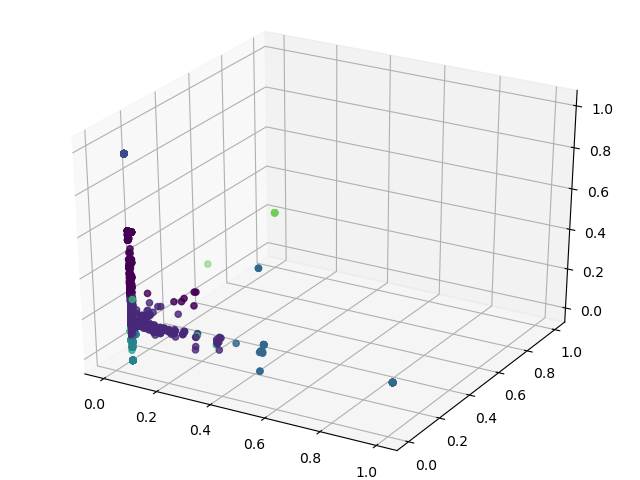
\includegraphics[height=0.3\paperwidth]{Figure_121.png}
    \caption{K-means聚类}
    \label{fig:kmeans}
\end{figure}


\begin{figure}
    \centering
    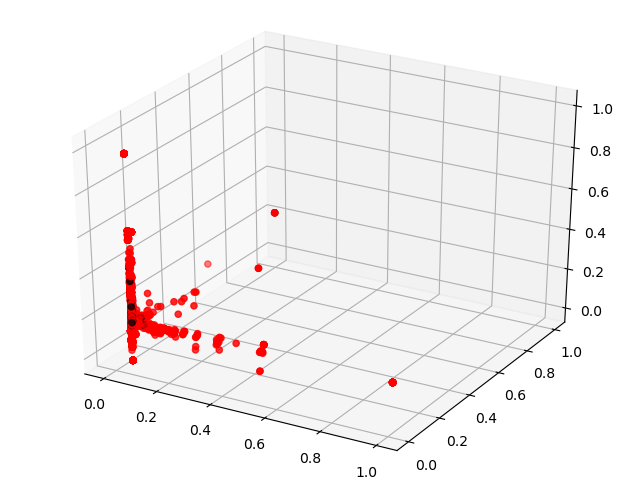
\includegraphics[height=0.3\paperwidth]{Figure_122.png}
    \caption{评分等级分类,黑色表示低评分,红色表示高评分}
    \label{fig:rating}
\end{figure}

\section{文档分类}

我们基于支持向量机对文档向量进行分类,预测评论的平行等级。抽取7000组数据作为训练集,将剩余的数据作为测试集,可以从
\autoref{fig:svm_y} 中看到,产品评级等级以5星和4星为主,总体上评星等级较高,预测结果正确率为0.53。
\begin{figure}
    \centering
    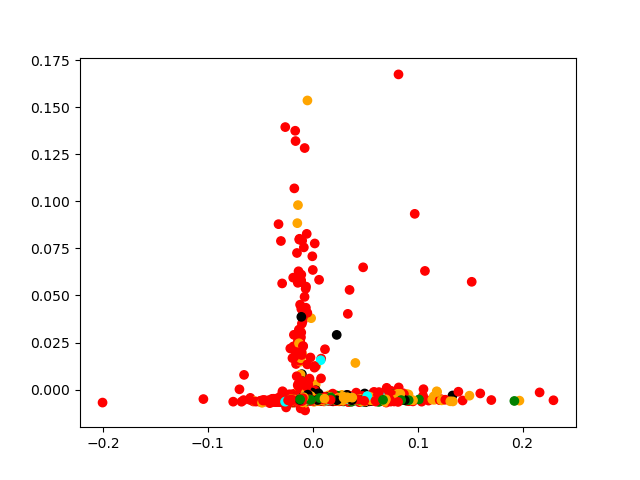
\includegraphics[height=0.3\paperwidth]{Figure_1.png}
    \caption{评论评星等级,红色代表5星,橙色代表4星,绿色代表3星,蓝色代表2星,黑色代表1星}
    \label{fig:svm_y}
\end{figure}

\section{时间序列分析预测评论量}

将数据进行整理得到月评论量,为了得到
平稳序列,对月评论量据进行2阶差分\autoref{fig:arima_diff},通过ADF检验
认为得到序列是平稳的。通过自相关图和偏自相关图\autoref{fig:arima_para}确定ARIMA的参数为
\begin{equation}
    p=12,d=2,q=0
\end{equation}

对ARIMA进行训练,将月评论量的后20个数据作为测试集,并与真实评论量做对比, 从\autoref{fig:arima_res} 中可以看出预测结果
在短期时预测结果与真实值接近,在较远的时间预测的趋势和真实评论量趋势一致.

\begin{figure}
    \centering
    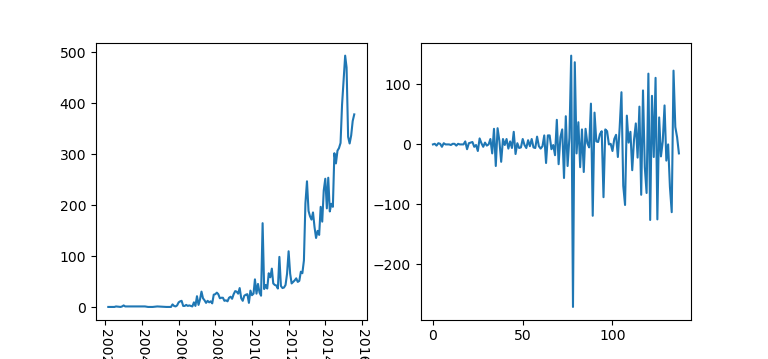
\includegraphics[width=1\textwidth]{diff.png}
    \caption{月销售数据和2阶差分结果}
    \label{fig:arima_diff}
\end{figure}

\begin{figure}
    \centering
    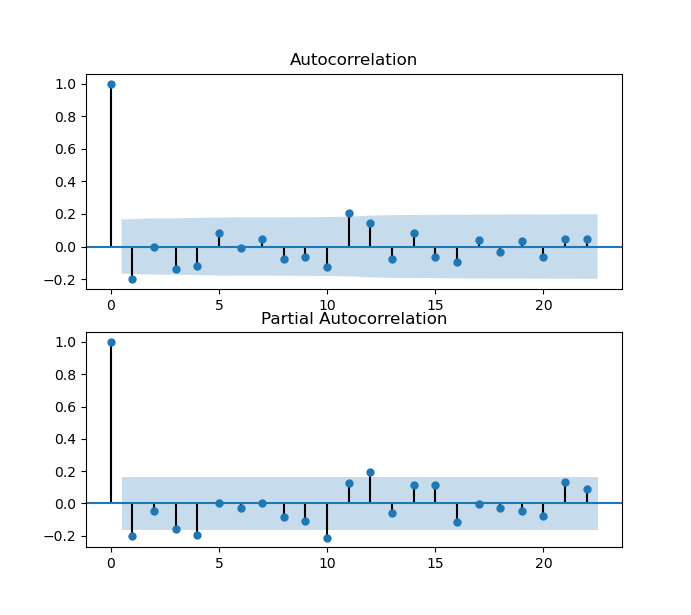
\includegraphics[width=1\textwidth]{acf_pacf.png}
    \caption{ACF PACF}
    \label{fig:arima_para}
\end{figure}

\begin{figure}
    \centering
    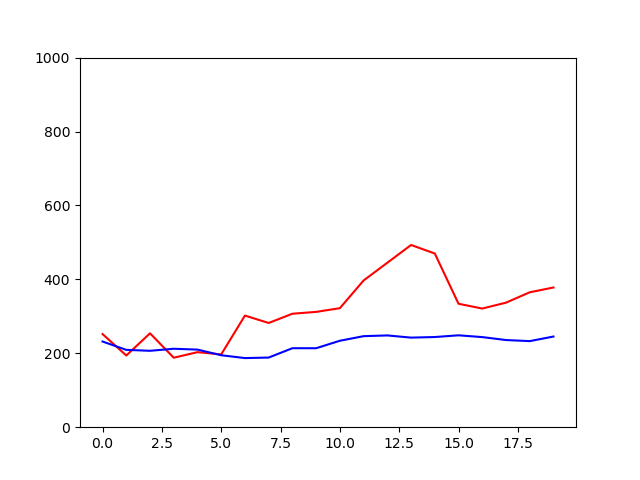
\includegraphics[height=0.3\paperwidth]{time_anal.png}
    \caption{ANIMA时间序列分析结果分析}
    \label{fig:arima_res}
\end{figure}

\chapter{讨论}
本次大作业基于亚马逊的在线市场为背景,希望我们能够通过使用一些数据科学的数学方法来完成对阳光
公司相关产品的一些预测与分析,在实践过程中,我们利用各种方法,采用了不同的模型来处理来自亚马
逊数据中心的用户评论数据集。首先,我们进行了对文件的预处理,获得了干净的而简洁的数据集,然后
这些数据来获得评论中的关键词,之后对文本信息进行向量化并且使用PCA进行降维处理,然后对完成了文
本聚类的操作并且还根据时间序列和评论的相关信息得到了一些更多的信息。

最终,我们得到了一些想要的结果并且完成了阳光公司的提出的问题,通过对这些结果进行分析,我们能够
像阳光公司提出一些建议。

此外,本次实践在对于文档分类的操作上还有可以提升的空间,目前我们达到了0.53准确率,但是如果
使用一些其他的算法,可能还有提升的空间。
